%%%%%%%%%%%%%%%%%%%%%%%%%%%%%%%%%%%%
%%                                %%
%%       Intra-node commn.        %%
%%                                %%
%%%%%%%%%%%%%%%%%%%%%%%%%%%%%%%%%%%%

\begin{frame}[fragile]
  \frametitle{Normal Charm++ semantics}
  \begin{itemize}
    \item Objects' memory buffers disjoint
    \item Communication involves copying of data
    \item Performance suffers when large arrays / non-linear data structures must be communicated
    \item Copying not strictly necessary for chares that share an address space
  \end{itemize}
\end{frame}

\begin{frame}[fragile]
  \frametitle{Intra-node communication}
  \begin{itemize}
    \item For objects sharing an address space, several mechanisms exist to reduce communication overhead
    \begin{itemize}
      \item Conditional packing
      \item PE-level data reuse through {\em groups}
      \item Logical node-level data reuse through {\em nodegroups}
    \end{itemize}
  \end{itemize}
\end{frame}

\begin{frame}[fragile]
  \frametitle{Conditional packing}
  \begin{itemize}
  \item Scenario
    \begin{itemize}
      \item Chare sending data array to multiple other chares
      \item Some neighbors might be on its logical node
      \item Neighbors access array in read-only fashion
    \end{itemize}
  \item Using ``normal'' Charm++ messages
    \begin{itemize}
      \item Create a varsize message
      \item Possibly copy data into message
      \item Invoke remote ({\em nokeep}) entry method with message
    \end{itemize}
  \item Requires copying even for same-node neighbors
  \end{itemize}
\end{frame}

\begin{frame}[fragile]
  \frametitle{Conditional packing}
  \begin{itemize}
  \item Alternative:
    \begin{itemize}
    \item Define {\em conditionally packed} data structure
    \item Maintains pointer to data array
    \item Has {\tt pup()} method, which is invoked by RTS only when data is crossing address space boundary
    \end{itemize}
  \item Same can be done for non-linear data structures, as long as proper {\tt pup()} method exists
  \end{itemize}
\end{frame}

\begin{frame}[fragile]
  \frametitle{Conditional packing schematic}
  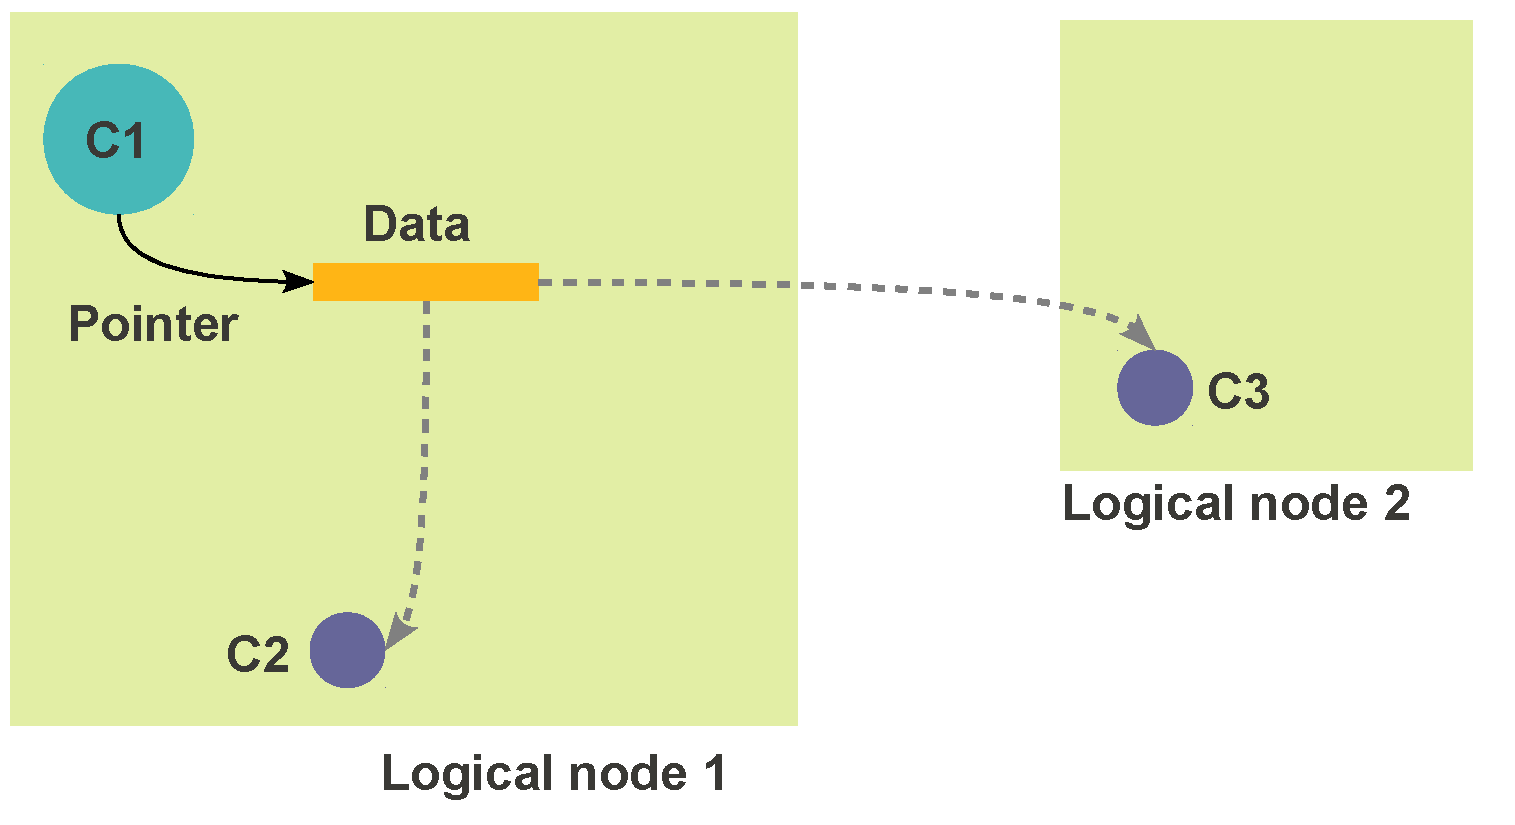
\includegraphics[width=\textwidth]{figures/advancedOpts/fig1}
\end{frame}

\begin{frame}[fragile]
  \frametitle{Conditional packing schematic}
  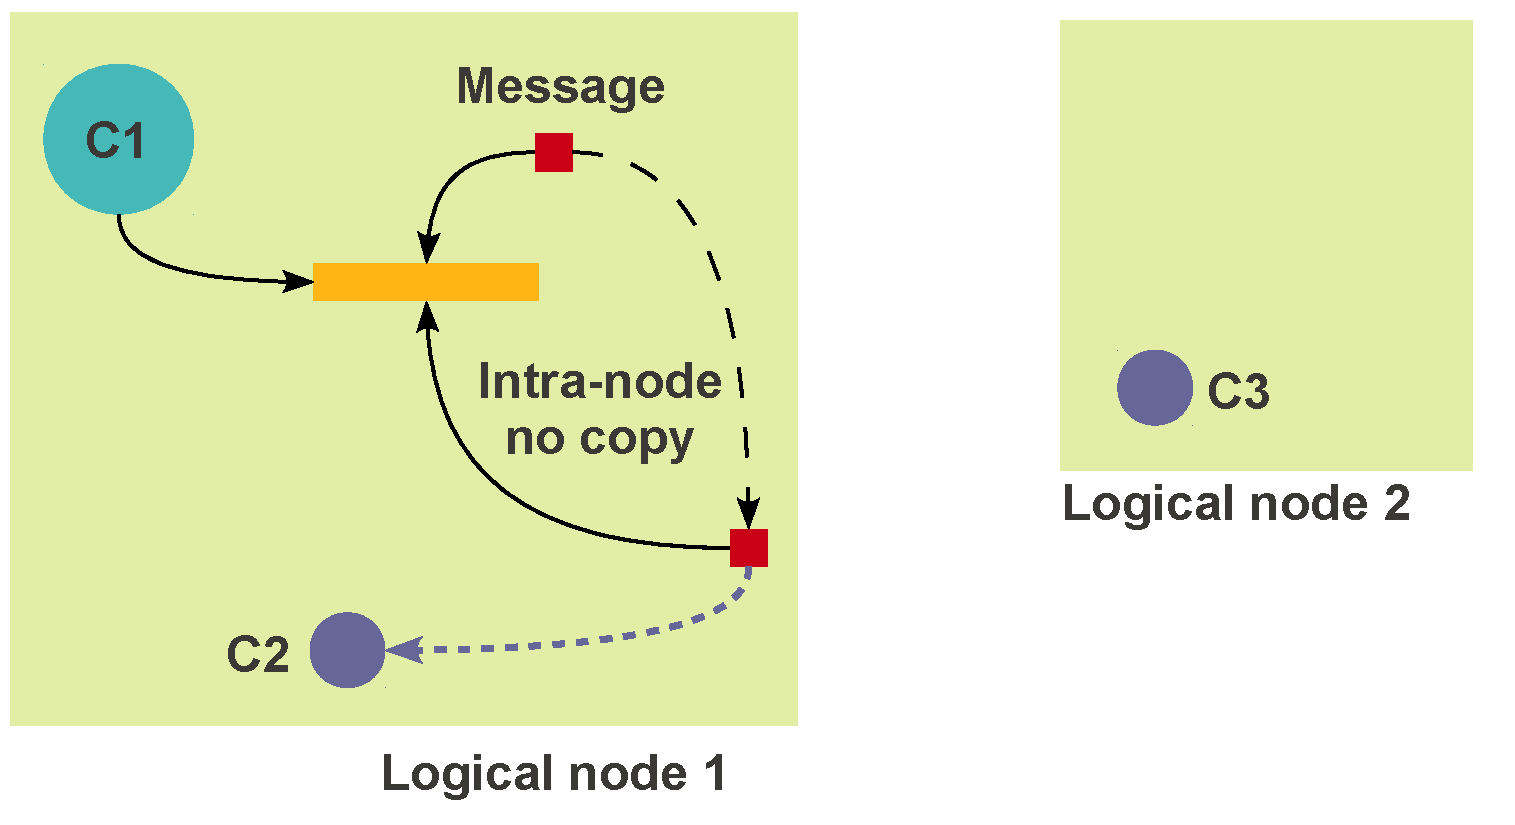
\includegraphics[width=\textwidth]{figures/advancedOpts/fig2}
\end{frame}

\begin{frame}[fragile]
  \frametitle{Conditional packing schematic}
  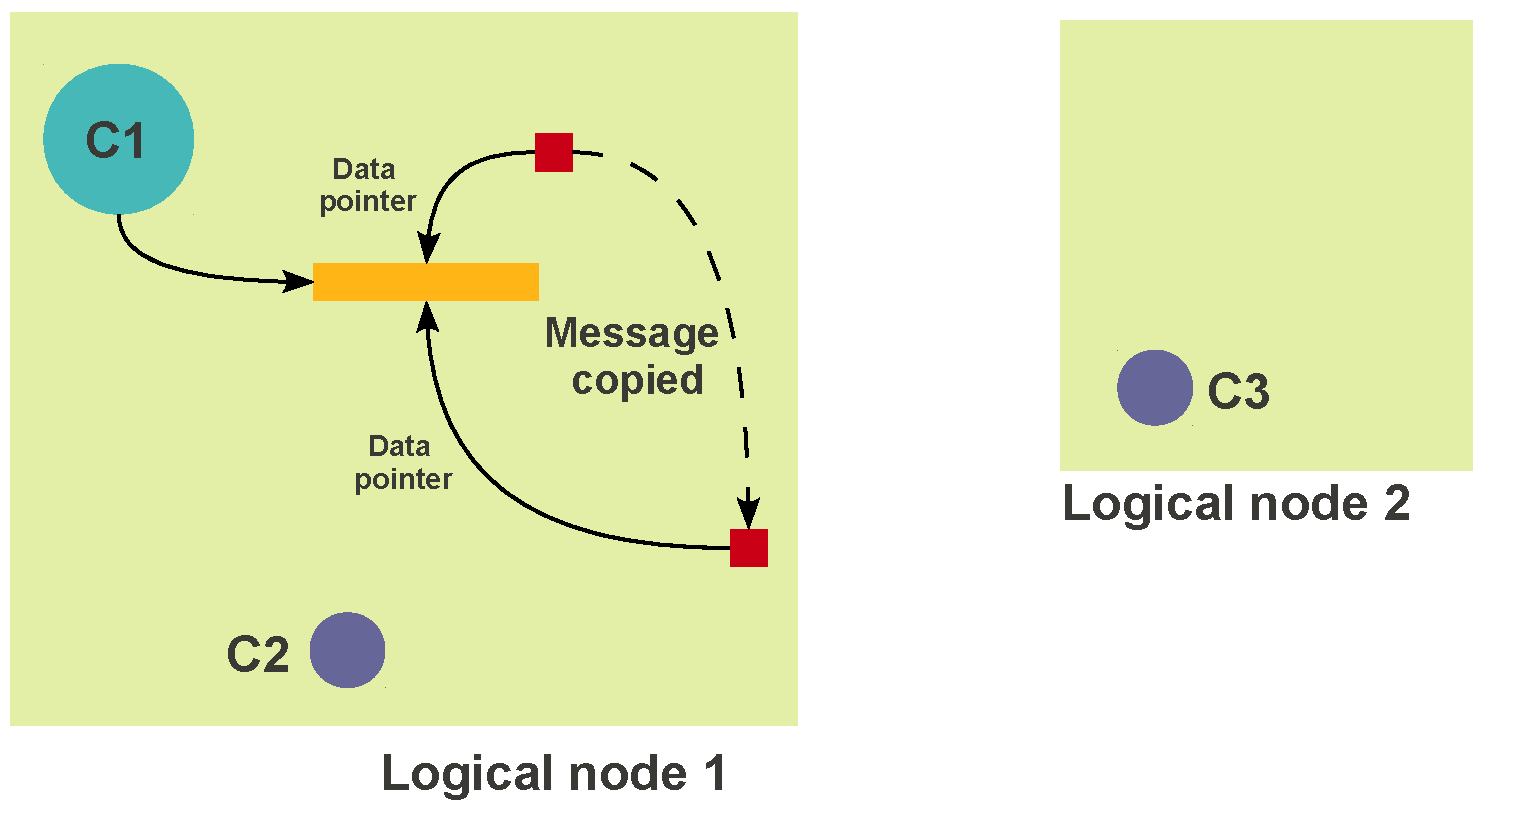
\includegraphics[width=\textwidth]{figures/advancedOpts/fig2_1}
\end{frame}

\begin{frame}[fragile]
  \frametitle{Conditional packing schematic}
  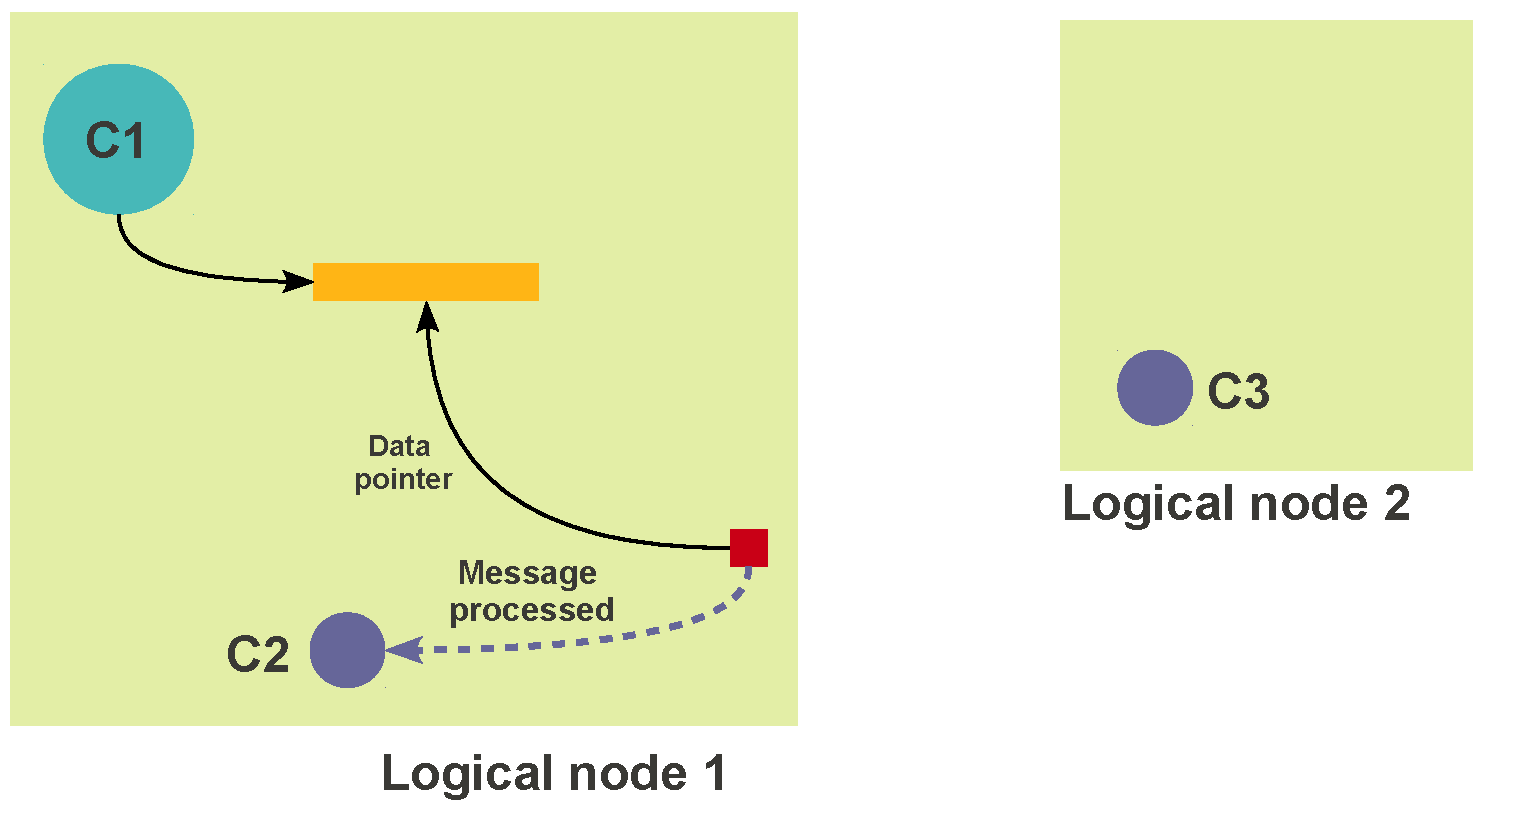
\includegraphics[width=\textwidth]{figures/advancedOpts/fig2_2}
\end{frame}

\begin{frame}[fragile]
  \frametitle{Conditional packing schematic}
  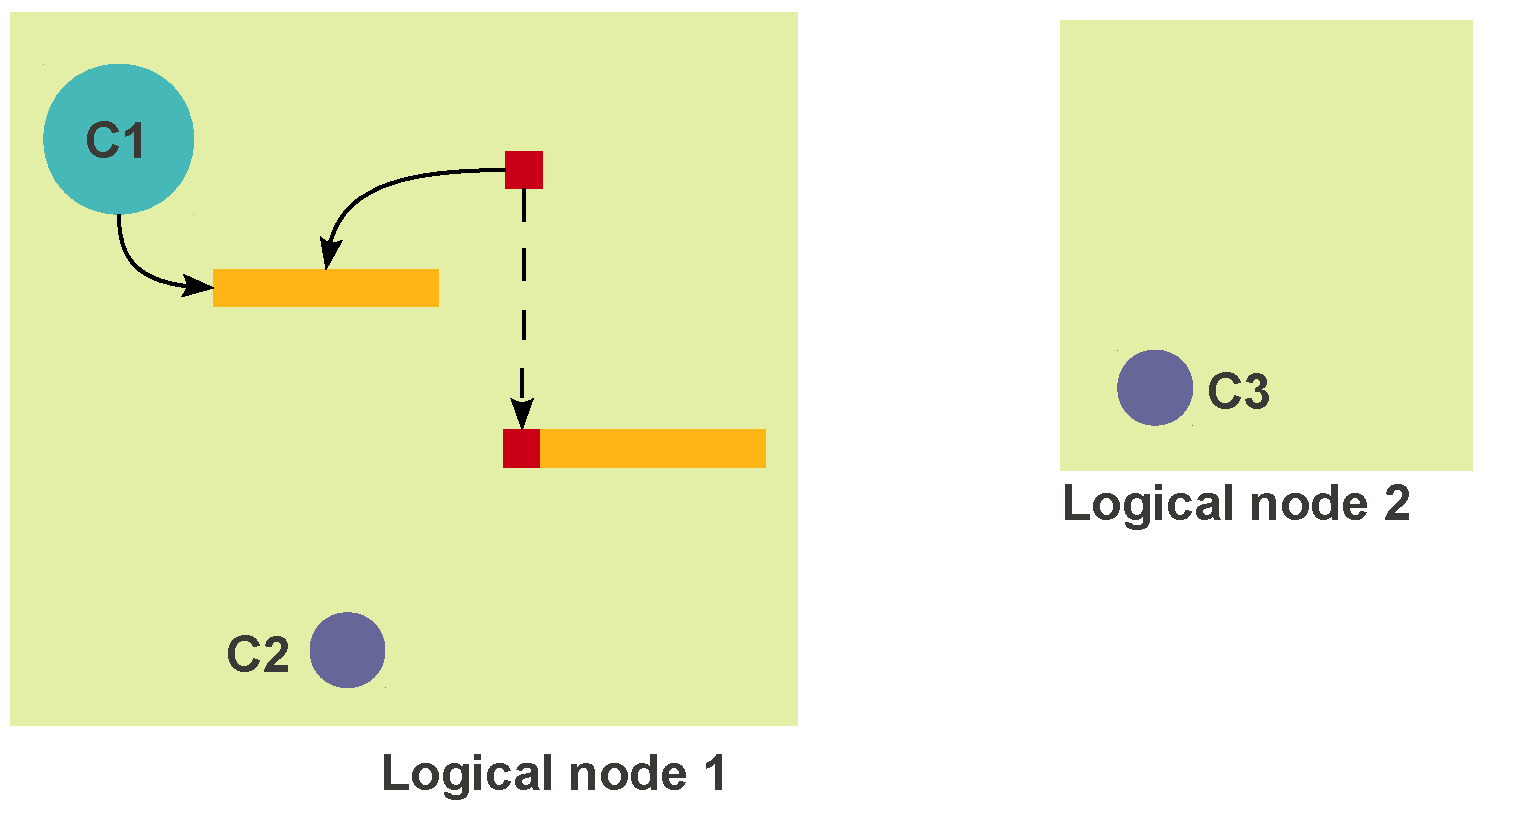
\includegraphics[width=\textwidth]{figures/advancedOpts/fig3}
\end{frame}

\begin{frame}[fragile]
  \frametitle{Conditional packing schematic}
  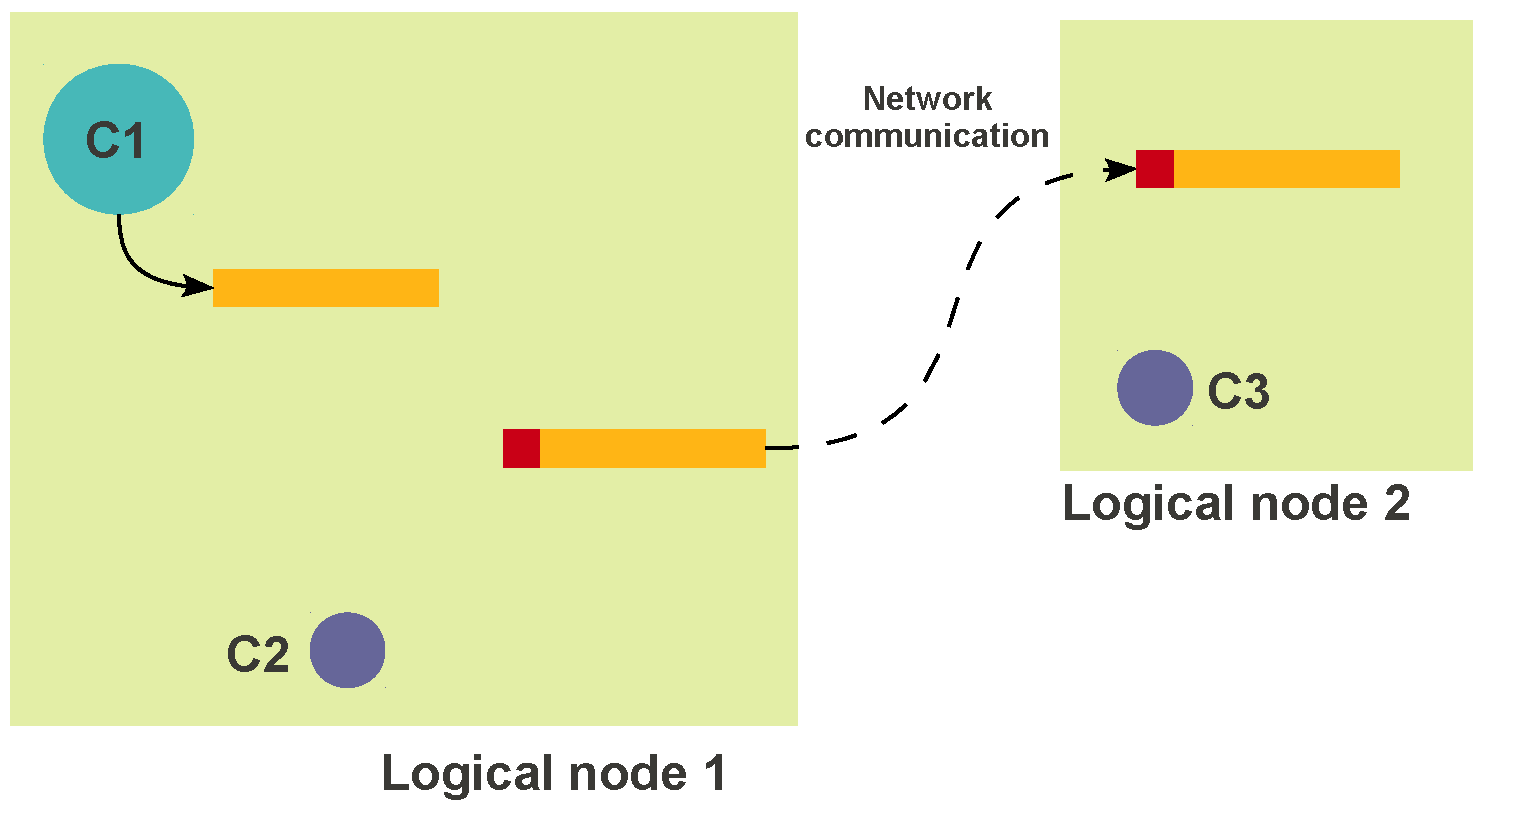
\includegraphics[width=\textwidth]{figures/advancedOpts/fig3_1}
\end{frame}

\begin{frame}[fragile]
  \frametitle{Conditional packing schematic}
  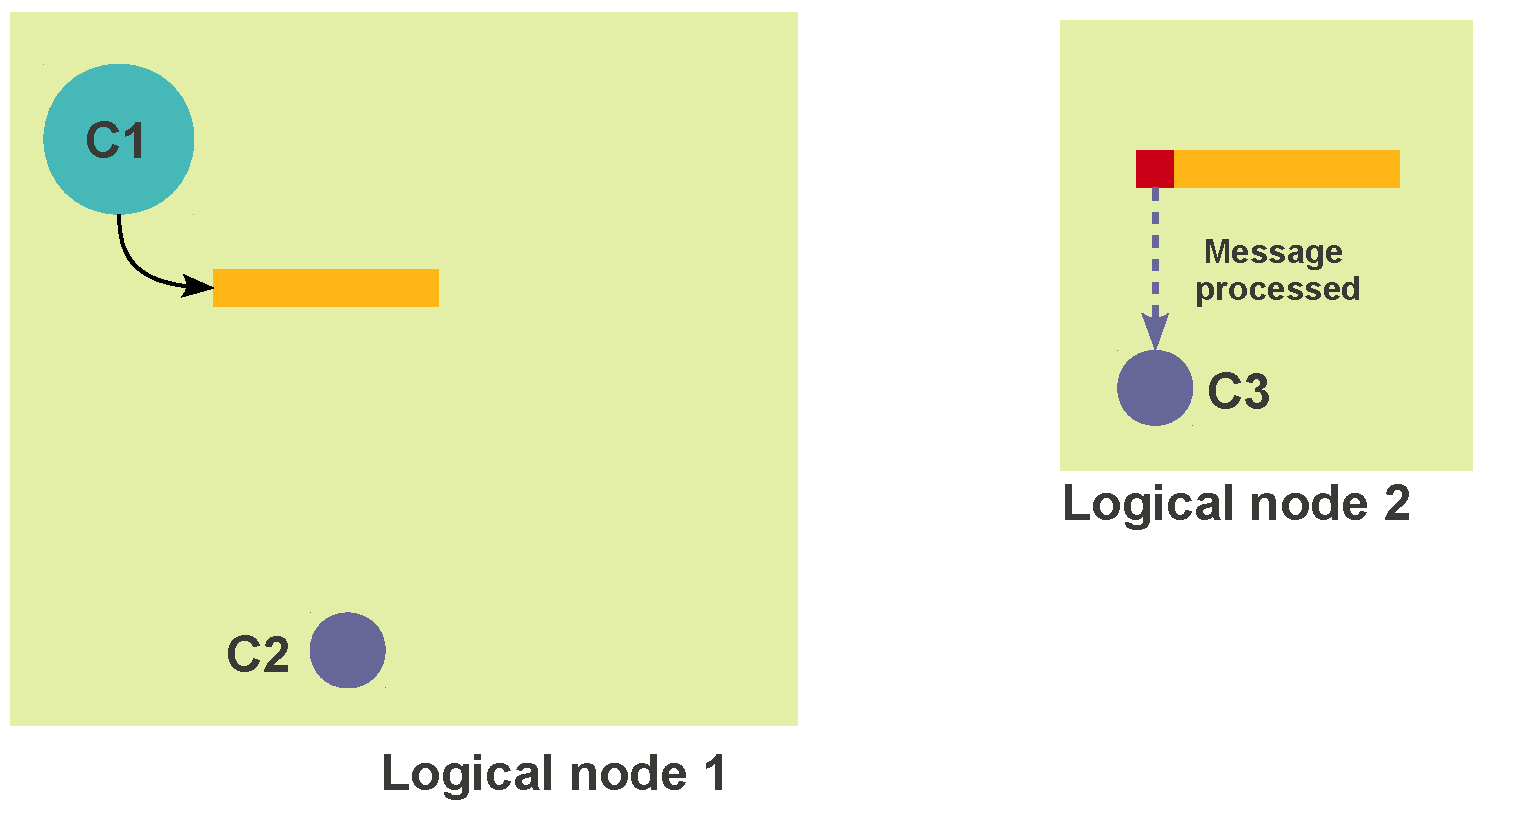
\includegraphics[width=\textwidth]{figures/advancedOpts/fig3_2}
\end{frame}

\begin{frame}[fragile]
  \frametitle{Sharing data between chares}
  \begin{itemize}
  \item Often applications have exhibit data reuse across chares on a PE
  \item Exploit this using Groups
  \item Pattern:
    \begin{itemize}
    \item Group local branch “owns” data, not chares
    \item Chares request group for data
    \item Via (local entry) methods defined on group
    \end{itemize}
  \end{itemize}
\end{frame}

\begin{frame}[fragile]
  \frametitle{Sharing data between chares: an example}
  \begin{itemize}
    \item Barnes-Hut type long-range $N$-body simulation
  \end{itemize}
  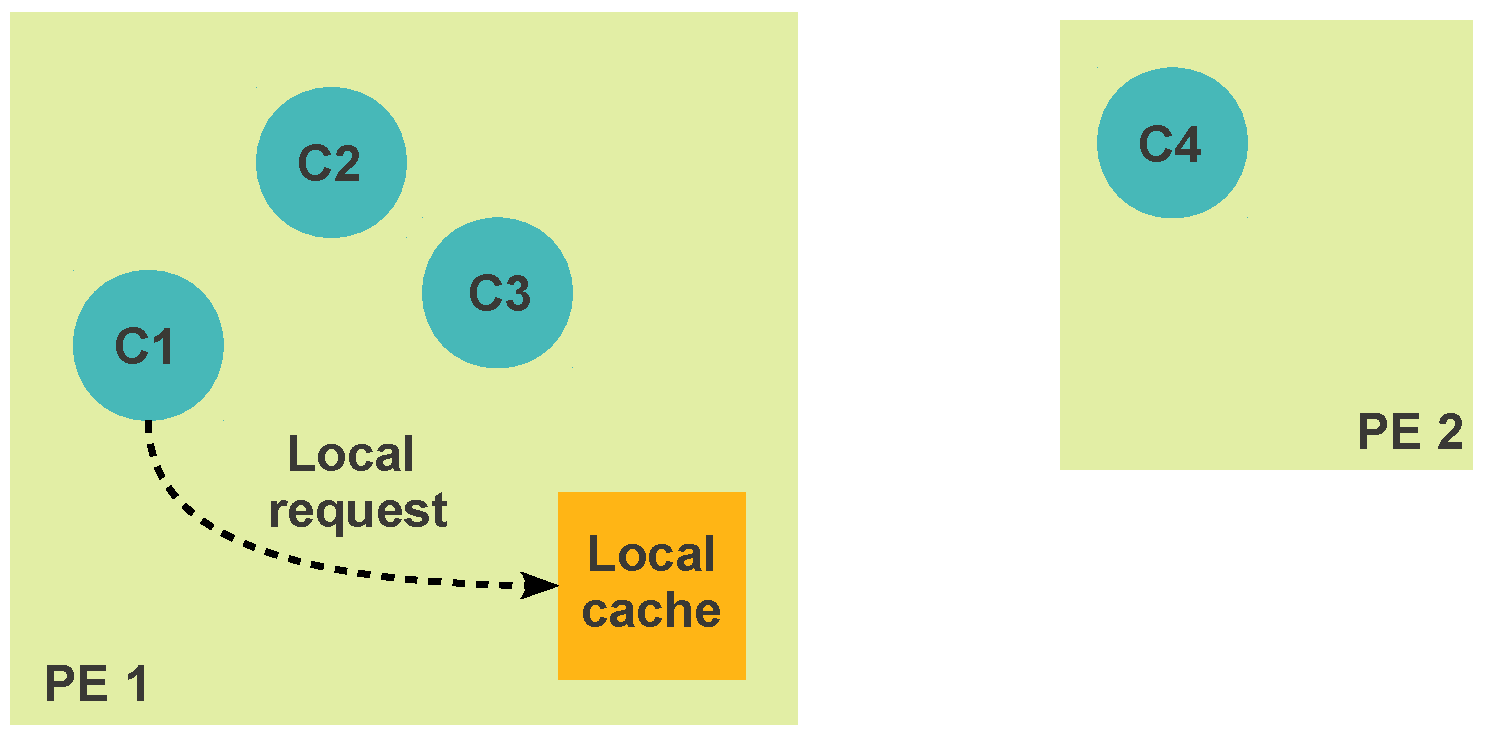
\includegraphics[width=\textwidth]{figures/advancedOpts/fig4}
\end{frame}

\begin{frame}[fragile]
  \frametitle{Sharing data between chares: an example}
  \begin{itemize}
    \item Barnes-Hut type long-range $N$-body simulation
  \end{itemize}
  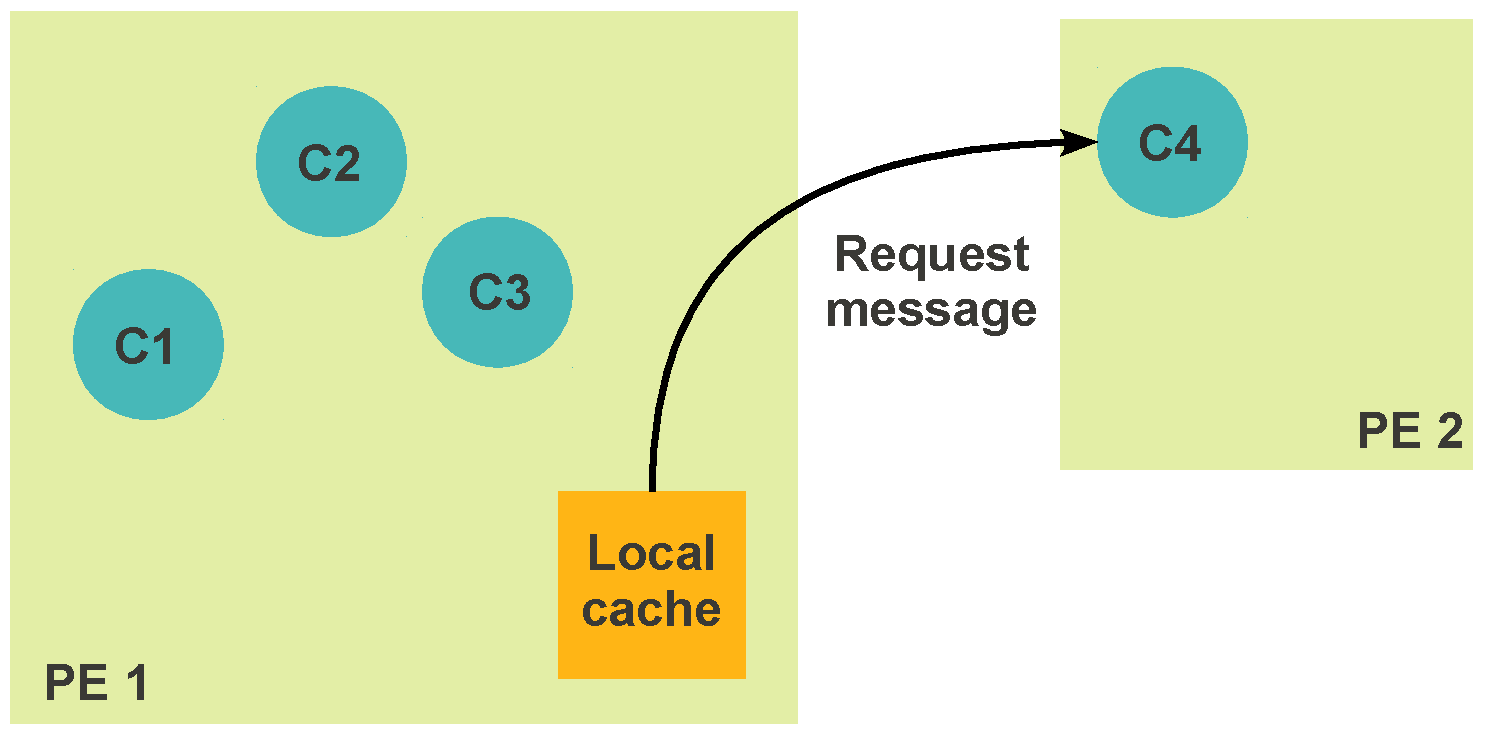
\includegraphics[width=\textwidth]{figures/advancedOpts/fig5}
\end{frame}

\begin{frame}[fragile]
  \frametitle{Sharing data between chares: an example}
  \begin{itemize}
    \item Barnes-Hut type long-range $N$-body simulation
  \end{itemize}
  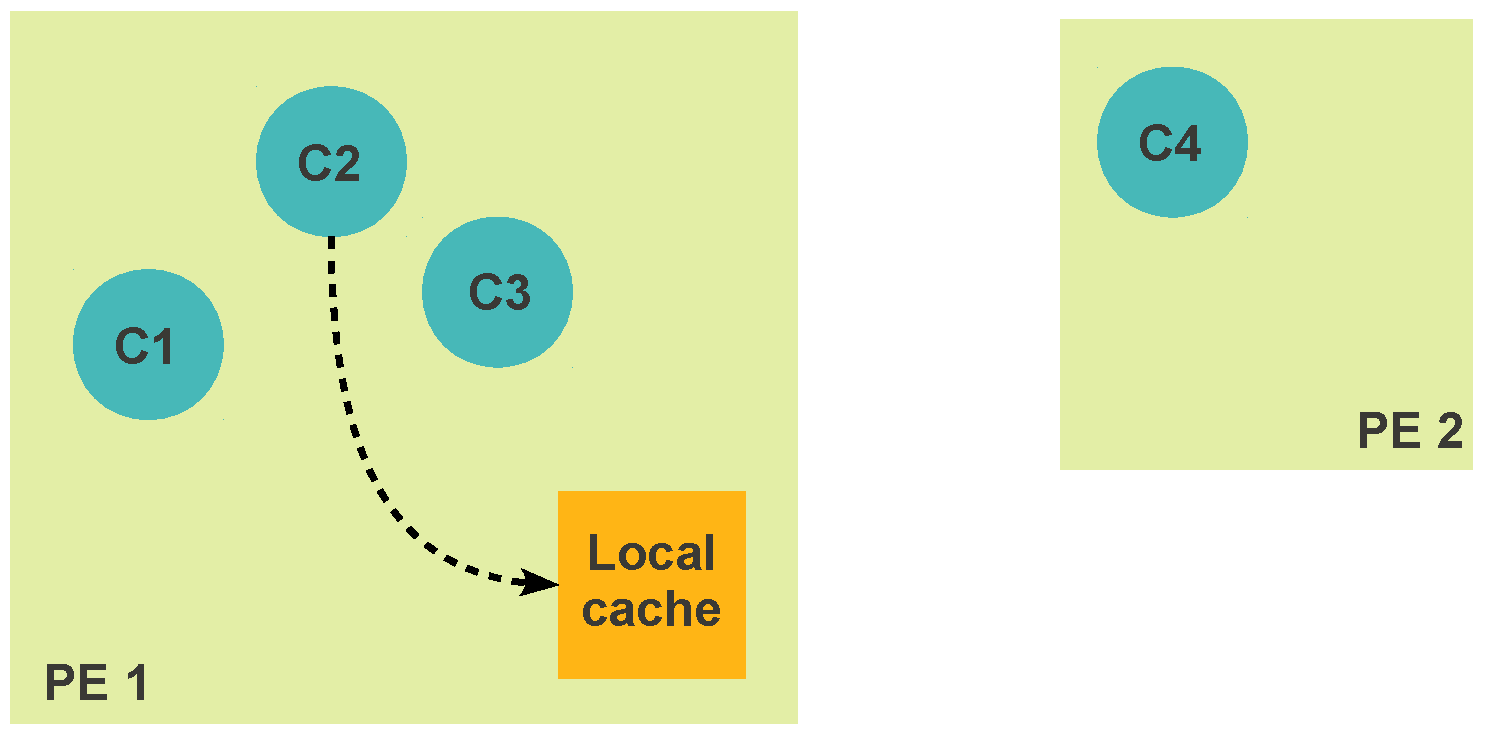
\includegraphics[width=\textwidth]{figures/advancedOpts/fig6}
\end{frame}

\begin{frame}[fragile]
  \frametitle{Sharing data between chares: an example}
  \begin{itemize}
    \item Barnes-Hut type long-range $N$-body simulation
  \end{itemize}
  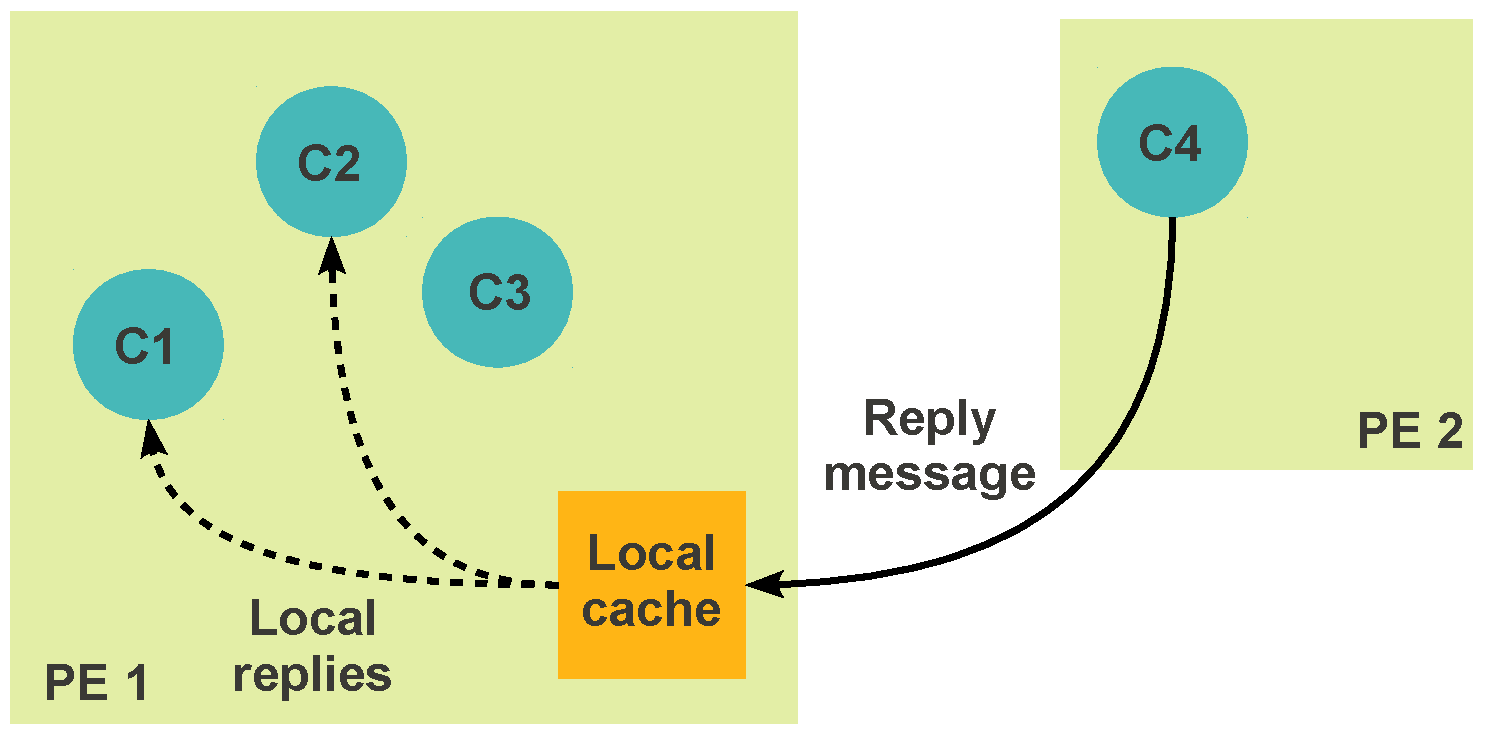
\includegraphics[width=\textwidth]{figures/advancedOpts/fig7}
\end{frame}

\begin{frame}[fragile]
  \frametitle{Sharing data between chares: an example}
  \begin{itemize}
    \item Barnes-Hut type long-range $N$-body simulation
  \end{itemize}
  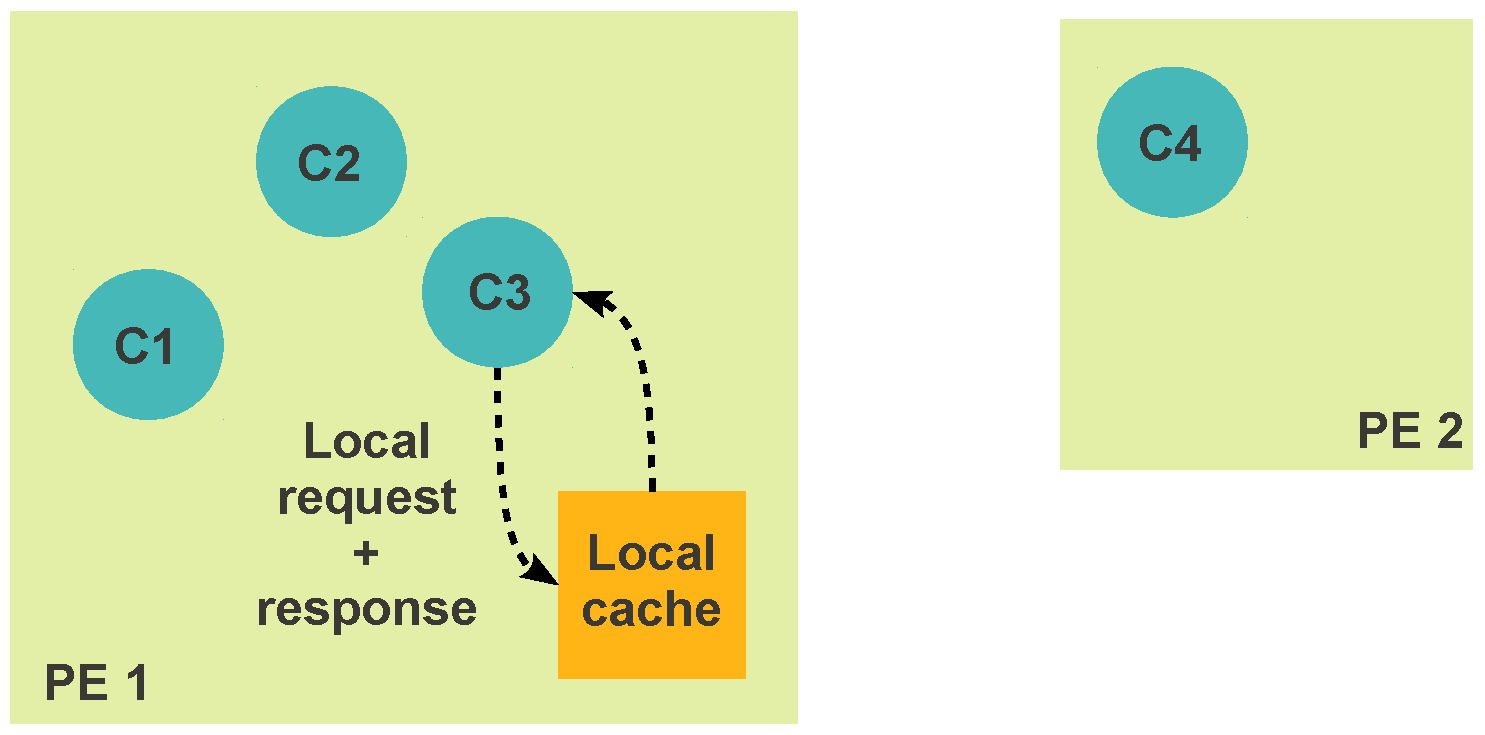
\includegraphics[width=\textwidth]{figures/advancedOpts/fig8}
\end{frame}

\begin{frame}[fragile]
  \frametitle{Sharing data between cores}
  \begin{itemize}
    \item In previous example, chares on same PE shared remotely fetched data
    \item Same idea can be used to share data across PEs on same logical node
    \item {\em Nodegroups}: one local branch per logical node
    \item {\bf Caution:}
    \begin{itemize}
      \item Nodegroup methods {\em not thread-safe} by default! 
      \item Use node-level locks for core synchronization
    \end{itemize}
  \end{itemize}
\end{frame}
